\setAuthor{Jaan Kalda}
\setRound{lahtine}
\setYear{2019}
\setNumber{G 7}
\setDifficulty{7}
\setTopic{Kinemaatika}

\prob{Külm gaas}
\begin{wrapfigure}[8]{r}{0.3\textwidth}
	\vspace{-5pt}
	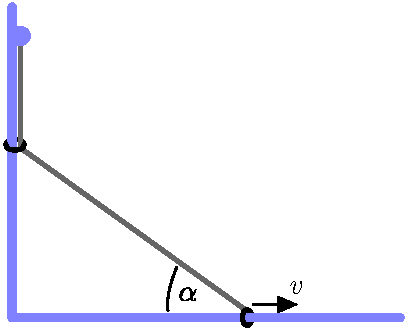
\includegraphics[width=0.3\textwidth]{2019-lahg-07-yl.pdf}
\end{wrapfigure}

Niit kogupikkusega $L$ on kinnitatud kahest üksteisega ristuvast lõigust koosneva relsi külge nii, nagu näidatud joonisel: üks niidi ots on fikseeritud jäigalt vertikaalse relsiosa külge kaugusele $h$ relsi nurgast, seejärel läheb niit läbi tillukese rõnga, mis saab libiseda mööda vertikaalset relssi ning niidi teine ots on kinnitatud tillukese rõnga kaudu horisontaalse relsi külge. Alumist rõngast hakatakse liigutatama konstantse kiirusega $v$. Leida teise rõnga kiirus ja kiirendus hetkel, mil nöör moodustab nurga $\alpha$ horisontaalsihiga.\hint
Üks lähenemisviisidest on tähistada alumise ja ülemise rõngaste kaugused nurgast vastavalt kui $x$ ja $y$. Sellisel juhul on $x$ ajaline tuletis $v$ ning otsitavad suurused on $y$ esimene ja teine ajaline tuletis.\solu
Alghetkel on molekulide vertikaalkiirus soojuskiirusest palju suurem. Molekulid lähenevad põhjale kiirusega $v$, seega lühikese ajavahemiku $t$ jooksul jõuavad põhjaga põrkuda molekulid ruumalast $vtS$, kus $S$ on põhja pindala, kogumassiga $\rho vtS$. Peale põrkumist lahkuvad nad kiirusega $v$, seetõttu said nad põhjalt koguimpulsi $\Delta p=2\rho v^2tS$. See vastab jõule $F=\Delta p/t$ ja rõhule $p=F/S=2\rho v^2$.

Pikema aja möödudes saavutavad molekulid soojusliku tasakaalu, st nende kiirusjaotus muutub isotroopseks ja algne kineetiline koguenergia muutub siseenergiaks: $U=V\rho v^2/2$, kus $V$ tähistab anuma ruumala. Teisest küljest,
\[
U=\frac 32 \frac{\rho V}\mu RT,
\]
millest $v^2=3 RT/\mu$ ning $p=\rho RT/\mu=\rho v^2/3$.\probend